\documentclass[tikz,border=5pt]{standalone}
\usepackage{amsmath}
\definecolor{curveblue}{HTML}{245C86}
\begin{document}
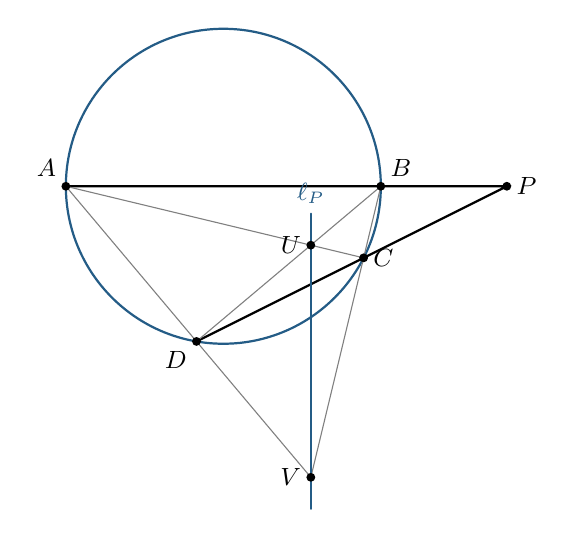
\begin{tikzpicture}[scale=2,font=\small,line cap=round]
\draw[curveblue,thick](0,0)circle(1);
\coordinate(A)at(-1.0000000,0.0000000);
\coordinate(B)at(1.0000000,0.0000000);
\coordinate(C)at(0.8906600,-0.4546700);
\coordinate(D)at(-0.1706600,-0.9853300);
\coordinate(P)at(1.8000000,0.0000000);
\coordinate(U)at(0.5555556,-0.3740834);
\coordinate(V)at(0.5555556,-1.8481388);
\draw[thick](A)--(P)--(D);
\draw[gray](A)--(U)--(C) (B)--(U)--(D) (A)--(V)--(D) (B)--(V)--(C);
\draw[curveblue,thick](0.5555556,-2.0481388)--(0.5555556,-0.1740834)node[above]{$\ell_P$};
\fill(A)circle(.8pt)node[above left]{$A$};
\fill(B)circle(.8pt)node[above right]{$B$};
\fill(C)circle(.8pt)node[right]{$C$};
\fill(D)circle(.8pt)node[below left]{$D$};
\fill(P)circle(.8pt)node[right]{$P$};
\fill(U)circle(.8pt)node[left]{$U$};
\fill(V)circle(.8pt)node[left]{$V$};
\end{tikzpicture}
\end{document}
